
\documentclass[fleqn,addpoints]{exam}

\usepackage{graphicx}
\usepackage{booktabs}
\usepackage{float}
\usepackage{amsmath}
\usepackage{cancel}
\usepackage{polynom}
\usepackage{caption}
\usepackage{mdwlist}

\newcommand{\degree}{\ensuremath{^\circ}} 

\printanswers

\ifprintanswers 
\usepackage{2in1, lscape} 
\fi

\title{Math 115 \\ Homework 25}
\date{May 31, 2011}

\begin{document}

\maketitle

% \begin{figure}[H]
%   \centering
%   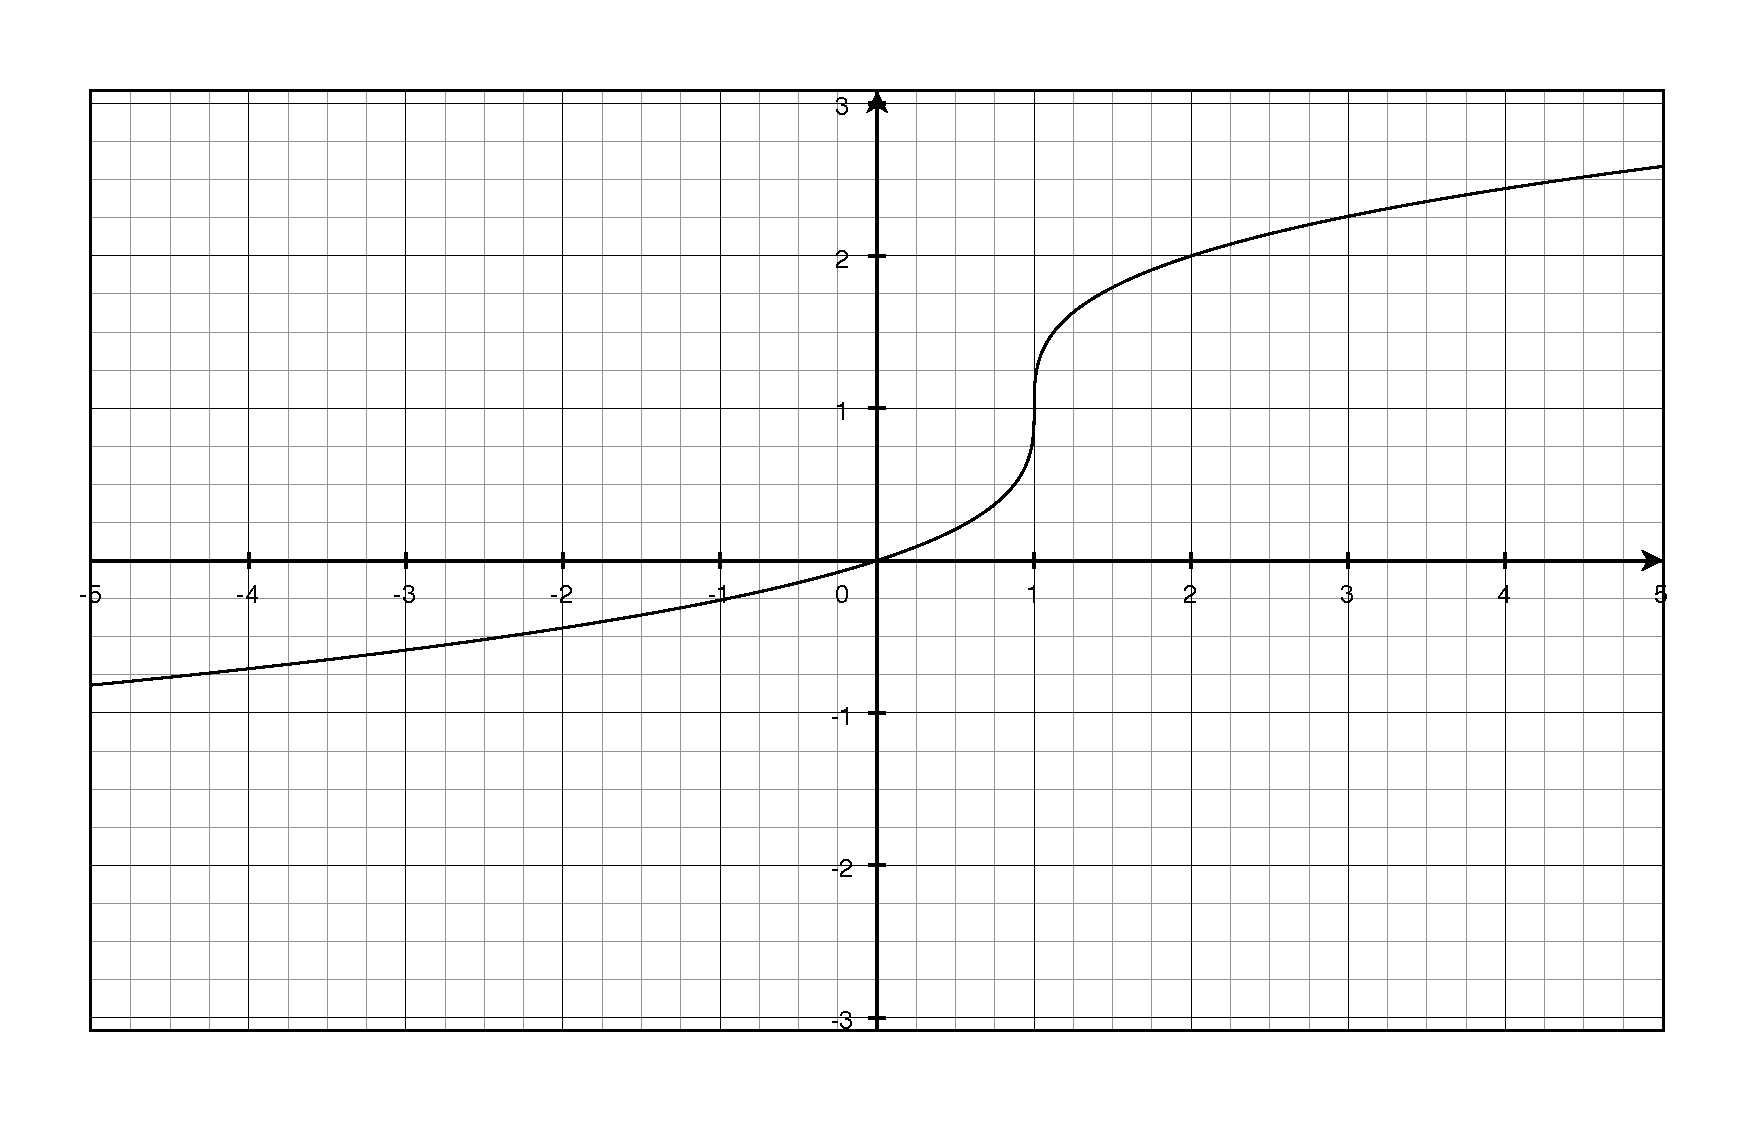
\includegraphics[scale=.3]{question7.eps}
%   \caption*{Question 7}
% \end{figure}

% \begin{tabular}{cc}
% \toprule
% period & amplitude \\
% \midrule
%   $\pi$ & $2$ \\
% \bottomrule
% \end{tabular}

\ifprintanswers
\else

\section{Administrative}

Good News--the predicted rapture came and went uneventfully, but for Math 115, The End is Near.  Here's the rough plan
for the next few weeks:

\begin{itemize*}
  \item May 31---Sections 5.4 and 5.5
  \item June 7---Sections 6.1 and 6.2
  \item June 14---Trigonometry Test
  \item June 21-June 28---Sections 10.2-10.4
  \item July---review and OU exam
\end{itemize*}

Section 5.3 doesn't seem to be included in the OU test, so in the interest of time, we'll skip it.  

\fi

\section{Homework}
\begin{itemize*}
  \item pp. 472-474: 1-2, 11-12, 23-24, 32-33, 41-42, 51-52, 55-56, 60, 61, 63, 77-80
  \item pp. 482-483: 1-5, 19-20, 23, 29, 31, 35-36, 45, 49, 55-56, 69, 97, 99, 123-124
\end{itemize*}

\section{Extra Credit}
Verify this identity:

\[
  \tan \left( \frac{\pi}{4} + \alpha \right)   \tan \left( \frac{\pi}{4} - \alpha \right) = 1
\]

\begin{solution}
\begin{align*}
  \tan \left( \frac{\pi}{4} - \theta \right) &= \frac{\tan \pi/4 - \tan \theta}{1 + \tan \pi/4 \tan \theta} \\
  &= \frac{1 - \tan \theta}{1 + \tan \theta}
\end{align*}

\begin{align*}
  \tan \left( \frac{\pi}{4} + \theta \right) &= \frac{\tan \pi/4 + \tan \theta}{1 - \tan \pi/4 \tan \theta} \\
  &= \frac{1 + \tan \theta}{1 - \tan \theta}
\end{align*}

Multiply them together:
\[
  \frac{\cancel{1 - \tan \theta}}{\cancel{1 + \tan \theta}} \cdot \frac{\cancel{1 + \tan \theta}}{\cancel{1 - \tan \theta}} = 1
\]

\end{solution}

\ifprintanswers
\section{Pages 447-449}

\begin{description}

\item[1] 
\begin{description}

\item[a]
\begin{align*}
  \cos \left( \frac{\pi}{4} + \frac{\pi}{3} \right) &= \cos \frac{\pi}{4} \cos \frac{\pi}{3} - \sin \frac{\pi}{4} \sin \frac{\pi}{3} \\
  &= \frac{\sqrt{2}}{2} \cdot \frac{1}{2} - \frac{\sqrt{2}}{2} \frac{\sqrt{3}}{2} \\
  &= \frac{\sqrt{2}}{4} - \frac{\sqrt{6}}{4} \\
  &= \frac{\sqrt{2} - \sqrt{6}}{4} \\
\end{align*}

\item[b]
\[
  \cos \frac{\pi}{4} + \cos \frac{\pi}{3} = \frac{\sqrt{2}}{2} + \frac{1}{2} = \frac{\sqrt{2} + 1}{2}
\]

\end{description}

\item[2] 
\begin{description}

\item[a]
\begin{align*}
  \sin \left( \frac{3\pi}{4} + \frac{5\pi}{6} \right) &= \sin \frac{3\pi}{4} \cos \frac{5 \pi}{6} + \cos \frac{3 \pi}{4} \sin \frac{5 \pi}{6} \\
  &= \frac{\sqrt{2}}{2} \cdot \left( - \frac{\sqrt{3}}{2} \right) + \left( -\frac{\sqrt{2}}{2} \right) \frac{1}{2} \\
  &= - \frac{\sqrt{6}}{4} - \frac{\sqrt{2}}{4} \\
  &= \frac{-\sqrt{2} - \sqrt{6}}{4} \\
\end{align*}

\item[b]
\[
  \sin \frac{3 \pi}{4} + \sin \frac{5 \pi}{6} = \frac{\sqrt{2}}{2} + \frac{1}{2} = \frac{\sqrt{2} + 1}{2}
\]

\end{description}

\item[11]
\begin{align*}
  \sin \frac{11 \pi}{12} &= \frac{\sqrt{6} - \sqrt{2}}{4} \\
  \cos \frac{11 \pi}{12} &= \frac{-\sqrt{6} - \sqrt{2}}{4} \\
  \tan \frac{11 \pi}{12} &= \frac{\sqrt{3} - \sqrt{3}}{\sqrt{3} + 3} = \frac{1 - \sqrt{3}}{1 + \sqrt{3}}  = \sqrt{3} - 2 \\
\end{align*}

\item[12]
\begin{align*}
  \sin \frac{7 \pi}{12} &= \frac{\sqrt{6} + \sqrt{2}}{4} \\
  \cos \frac{7 \pi}{12} &= \frac{\sqrt{2} - \sqrt{6}}{4} \\
  \tan \frac{7 \pi}{12} &= \frac{1 + \sqrt{3}}{1 - \sqrt{3}} = -\sqrt{3} - 2 \\
\end{align*}

\item[23]
\[
  \cos 25 \degree \cos 15 \degree - \sin 25 \degree \sin 15 \degree = \cos(25 \degree + 15 \degree) = \cos 40 \degree
\]

\item[24]
\[
  \sin 140 \degree \cos 50 \degree + \cos 140 \degree \sin 50 \degree = \sin(140 \degree + 50 \degree) = \sin 190 \degree
\]

\item[32]
\begin{align*}
  \cos 15 \degree \cos 60 \degree + \sin 15 \degree \sin 60 \degree &= \cos (15 \degree -  60 \degree) \\
  &= \cos (- 45 \degree) \\
  &= \cos 45 \degree \\
  &= \frac{\sqrt{2}}{2} \\
\end{align*}

\item[33]
\begin{align*}
  \sin \frac{\pi}{12} \cos \frac{\pi}{4} + \cos \frac{\pi}{12} \sin \frac{\pi}{4} &= \sin \left (\frac{\pi}{12} + \frac{\pi}{4} \right) \\
    &= \sin \left( \frac{\pi}{3} \right) \\
    &= \frac{\sqrt{3}} {2} \\
\end{align*}

\item[41]
\[
  \tan(u + v) = - \frac{63}{16} \\
\]

\item[42]
\[
  \csc(u-v) = \frac{65}{33}
\]

\item[51]
\begin{align*}
  \sin(u+v) &= x^2 + (\sqrt{1-x^2})^2  \\
  &= x^2 + 1 - x^2 \\
  &= 1 \\
\end{align*}

\item[52]
\begin{align*}
  \sin(u-v) &= \frac{2x}{\sqrt{1 + 4x^2}} \cdot x - \frac{1}{\sqrt{1 + 4x^2}} \cdot \sqrt{1-x^2} \\
  &= \frac{2x^2 - \sqrt{1 - x^2}}{4x^2 + 1} \\
\end{align*}

\item[55]
\begin{align*}
  \sin(3 \pi - x) &= \sin 3 \pi \cos x - \cos 3 \pi \sin x \\
  &= 0 - (-1)(\sin x) \\
  &= \sin x \\
\end{align*}

\item[56]
\begin{align*}
  \sin \left( \frac{\pi}{2} + x \right) &= \sin \frac{\pi}{2} \cos x + \cos \frac{\pi}{2} \sin x \\
  &= \cos x + 0 \\
  &= \cos x \\
\end{align*}

\item[60]
\begin{align*}
  \tan \left( \frac{\pi}{4} - \theta \right) &= \frac{\tan \pi/4 - \tan \theta}{1 + \tan \pi/4 \tan \theta} \\
  &= \frac{1 - \tan \theta}{1 + \tan \theta}
\end{align*}

\item[61]
\begin{align*}
  \cos(x &+ y) \cos(x-y) \\
  &= (\cos x \cos y - \sin x \sin y)(\cos x \cos y + \sin x \sin y) \\
  &= \cos^2 x \cos^2 y - \sin^2 x \sin^2 y \\
  &= \cos^2 x (1 - \sin^2 y) - (1 - \cos^2 x) \sin^2 y \\
  &= \cos^2 x - \cos^2 x \sin^2 y - (\sin^2 y - \cos^2x \sin^2 y) \\
  &= \cos^2 x - \sin^2 y \\
\end{align*}

\item[63]
\begin{align*}
  \sin(x+y) &+ \sin(x-y) \\
  &= \sin x \cos y + \cos x \sin y + \sin x \cos y - \cos x \sin y \\
  &= 2 \sin x \cos y \\
\end{align*}

\item[77]
false.  If, for example, $u = v = \dfrac{\pi}{4}$ then $\sin(u + v) = 1$ and $\sin u + \sin v = \sqrt{2}$

\item[78]
false.  If, for example, $u = v = \dfrac{\pi}{4}$ then $\cos(u + v) = 0$ and $\cos u + \cos v = \sqrt{2}$

\item[79]
false

\begin{align*}
  \cos \left( x - \frac{\pi}{2} \right) &= \cos x \cos \frac{\pi}{2} + \sin x \sin \frac{\pi}{2} \\
  &= 0 + \sin x \\
  &= \sin x \\
\end{align*}

\item[80]
true

\begin{align*}
  \sin \left( x - \frac{\pi}{2} \right) &= \sin x \cos \frac{\pi}{2} - \cos x \sin \frac{\pi}{2} \\
  &= 0 - \cos x \\
  &= -\cos x \\
\end{align*}

\section{Pages 482-483}

\item[1]
\[
  \frac{\sqrt{17}}{17}
\]

\item[2]
\[
  \frac{1}{4}
\]

\item[3]
\[
  \cos 2 \theta = 1 - 2 \sin^2 \theta = \frac{15}{17}
\]

\item[4]
\[
  \sin 2 \theta =  2 \sin \theta \cos \theta = \frac{8}{17}
\]

\item[5]
\[
  \tan 2 \theta =  \frac{2 \tan \theta}{1 - \tan^2 \theta} = \frac{8}{15}
\]

\item[19]
\[
  6 \sin x \cos x = 3 (2 \sin x \cos x) = 3 \sin 2x
\]

\item[20]
\[
  6 \cos^2 x - 3 = 3(2 \cos^2 x - 1) = 3 \cos 2x 
\]

\item[23]
\begin{align*}
  \sin 2u &= 2 \left( - \frac{4}{5} \right) \left( - \frac{3}{5} \right) = \frac{24}{25} \\
  \cos 2u &= 2 \left( - \frac{3}{5} \right)^2 - 1 = - \frac{7}{25} \\
  \tan 2u &= \frac{2 (4/3)}{1 - 16/9} = - \frac{24}{7} \\
\end{align*}

\item[29]
\begin{align*}
  \cos^4 x &= (\cos^2 x)^2 \\
  &= \left( \frac{1 + \cos 2x}{2} \right)^2 \\
  &= \frac{1 + 2 \cos 2x + \cos^2 2x}{4} \\
  &= \cfrac{1 + 2 \cos 2x + \cfrac{1 + \cos 2x}{2}}{4} \\
  &= \frac{3 + 4 \cos 2x + \cos 4x}{8} \\
\end{align*}

\item[31]
\begin{align*}
  \sin^2 x \cos^2 x &= \left( \frac{1 - \cos 2x}{2} \right) \left( \frac{1 + \cos 2x}{2} \right) \\
  &= \frac{1 - \cos^2 2x}{4} \\
  &= \frac{1 - \left( \cfrac{1 + \cos 4x}{2} \right) }{4} \\
  &= \frac{1 - \cos 4x}{8} \\
\end{align*}

\item[35]
\[
  \cos \frac{\theta}{2} = \sqrt{\frac{1 + \cos \theta}{2}} = \frac{4 \sqrt{17}}{17}
\]

\item[36]
\[
  \sin \frac{\theta}{2} = \sqrt{\frac{1 - \cos \theta}{2}} = \frac{\sqrt{17}}{17}
\]

\item[45]
\begin{align*}
  \sin \frac{\pi}{8} &= \sqrt{\frac{1 - \cos \pi/4}{2}} = \frac{\sqrt{2 - \sqrt{2}}}{2} \\
  \cos \frac{\pi}{8} &= \sqrt{\frac{1 + \cos \pi/4}{2}} = \frac{\sqrt{2 + \sqrt{2}}}{2} \\
  \tan \frac{\pi}{8} &= \frac{\sin \pi/4}{1 + \cos \pi/4} = \frac{\sqrt{2}}{2 + \sqrt{2}} = \frac{1}{\sqrt{2} + 1} = \sqrt{2} - 1 \\
\end{align*}

\item[49]
\begin{align*}
  \sin \frac{u}{2} &= \sqrt{ \frac{1 - \cos u}{2} } = \frac{5 \sqrt{26}}{26} \\
  \cos \frac{u}{2} &= \sqrt{ \frac{1 + \cos u}{2} } = \frac{\sqrt{26}}{26} \\
  \tan \frac{u}{2} &= \frac{\sin u}{1 + \cos u} = 5 \\
\end{align*}

\item[55]
\[
  \sqrt{\frac{1 - \cos 6x}{2}} = |\sin 3x|
\]

\item[56]
\[
  \sqrt{\frac{1 + \cos 4x}{2}} = |\cos 2x|
\]

\item[69]
\begin{align*}
  \sin(x &+y) \sin(x-y) \\
  &= \frac{1}{2} ( \cos(x+y - (x-y)) - \cos(x+y+x-y) ) \\
  &= \frac{1}{2} (\cos 2y - \cos 2x) \\
\end{align*}

\item[97]
\begin{align*}
  \cos^2 2 \alpha - \sin^2 2 \alpha &= \frac{1 + \cos 4 \alpha}{2} - \frac{1 - \cos 4 \alpha}{2} \\
  &= \frac{2 \cos 4 \alpha}{2} \\
  &= \cos 4 \alpha \\
\end{align*}

\item[99]
\begin{align*}
  (\sin x + \cos x)^2 &= \sin^2 x + \cos^2 x + 2 \sin x \cos x \\
  &= 1 + 2 \sin x \cos x \\
  &= 1 + \sin 2x \\
\end{align*}

\item[123]
false

\item[124]
false.  The thing that matters is what quadrant $\dfrac{u}{2}$ is in.  

\end{description}

\else

\vspace{2 in}

\begin{em}
  A man is rich in proportion to the number of things he can afford to let alone.
\end{em}

\vspace{.2 cm}
\hspace{1.5 cm} --Henry David Thoreau

\fi

\end{document}

